\documentclass[conference]{IEEEtran}
\IEEEoverridecommandlockouts
% The preceding line is only needed to identify funding in the first footnote. If that is unneeded, please comment it out.
\usepackage{cite}
\usepackage{amsmath,amssymb,amsfonts}
\usepackage{algorithmic}
\usepackage{graphicx}
\usepackage{textcomp}
\usepackage{xcolor}
\def\BibTeX{{\rm B\kern-.05em{\sc i\kern-.025em b}\kern-.08em
    T\kern-.1667em\lower.7ex\hbox{E}\kern-.125emX}}
\begin{document}

\title{Classification of Red Wine Quality using Various Machine Learning Algorithms}

\author{\IEEEauthorblockN{1\textsuperscript{st} Haoyu Quan}
\IEEEauthorblockA{\textit{ Mckelvey School of Engineering} \\
\textit{Washington University in St. Louis}\\
St. Louis, MO \\
quanhaoyu@wustl.edu}
\and
\IEEEauthorblockN{2\textsuperscript{nd} Anny Qiao}
\IEEEauthorblockA{\textit{ Mckelvey School of Engineering} \\
\textit{Washington University in St. Louis}\\
St. Louis, MO \\
a.qiao@wustl.edu}
\and
\IEEEauthorblockN{3\textsuperscript{rd} Bruce Li}
\IEEEauthorblockA{\textit{ Mckelvey School of Engineering} \\
\textit{Washington University in St. Louis}\\
St. Louis, MO \\
liyifei@wustl.edu}
}

\maketitle
\begin{abstract}
	This study implemented three machine learning classification methods, KNN, SVM, and Random Forest, on the UCI red-wine dataset to classify wines. Results showed that the KNN method had the lowest performance with an accuracy of 61.97$\%$ and an MSE of 0.4985, while the SVM method performed better with an accuracy of 65.87$\%$ and an MSE of 0.4678. The Random Forest method achieved the highest accuracy of 75$\%$ and the lowest MSE of 0.35. The study highlights the importance of data cleaning and standardization in improving the accuracy and MSE of machine learning models. The findings suggest that the Random Forest method is the most effective approach for wine classification.
\end{abstract}
\section{Introduction}
Machine learning is a branch of artificial intelligence that enables machines to learn from data and make predictions or decisions without being explicitly programmed. It finds applications in a wide range of domains such as image recognition, natural language processing, and predictive modeling. In this project, we aim to use supervised machine learning algorithms to classify a wine quality data set based on 11 given features. While wine was once viewed as a luxury good, it is now enjoyed by a wider range of consumers. Quality evaluation is a crucial part of the certification process and can help to identify influential factors during the wine production process.\cite{b1}In our project, these factors will be used as features for our machine learning algorithm.

The primary objective of this project is to build a machine learning model that can accurately predict the quality of wine into 10 different levels with the given data. Furthermore, we aim to compare the performance of different machine learning algorithms such as Support Vector Machines (SVM), K-Nearest Neighbors (KNN), and Random Forest to determine the most effective algorithm for this task. To improve the accuracy of our model, we have implemented various methods of data cleaning, chosen optimal weight factors, and tuned other hyperparameters.

After multiple testing and trial and error iterations, the model was able to achieve an accuracy rate of over 60 percent. Overall, this project demonstrates the effectiveness of supervised machine learning algorithms in predicting the quality of wine based on various influential factors during the production process.\\

\section{Methods}
\subsection{Exploratory Data Analysis}


The dataset used in this project was introduced by Cortez et al.\cite{b2}

The dataset is a collection of 1599 samples, each representing a different red wine, with 11 physicochemical attributes that describe the properties of the wine accompanied with a quality rating. These attributes includes but not limited to: amount of various acid, residual sugar, chlorides, sulfates in the wine; density; pH value; alcohol content; etc. The quality rating is scored as an integer between 0 and 9.

As the original research aims to find which chemical properties influence the quality of red wines, we here focus on analyzing the column of wine quality.


	\begin{figure}[h]
	\label{fig:foo}
	\begin{center}
	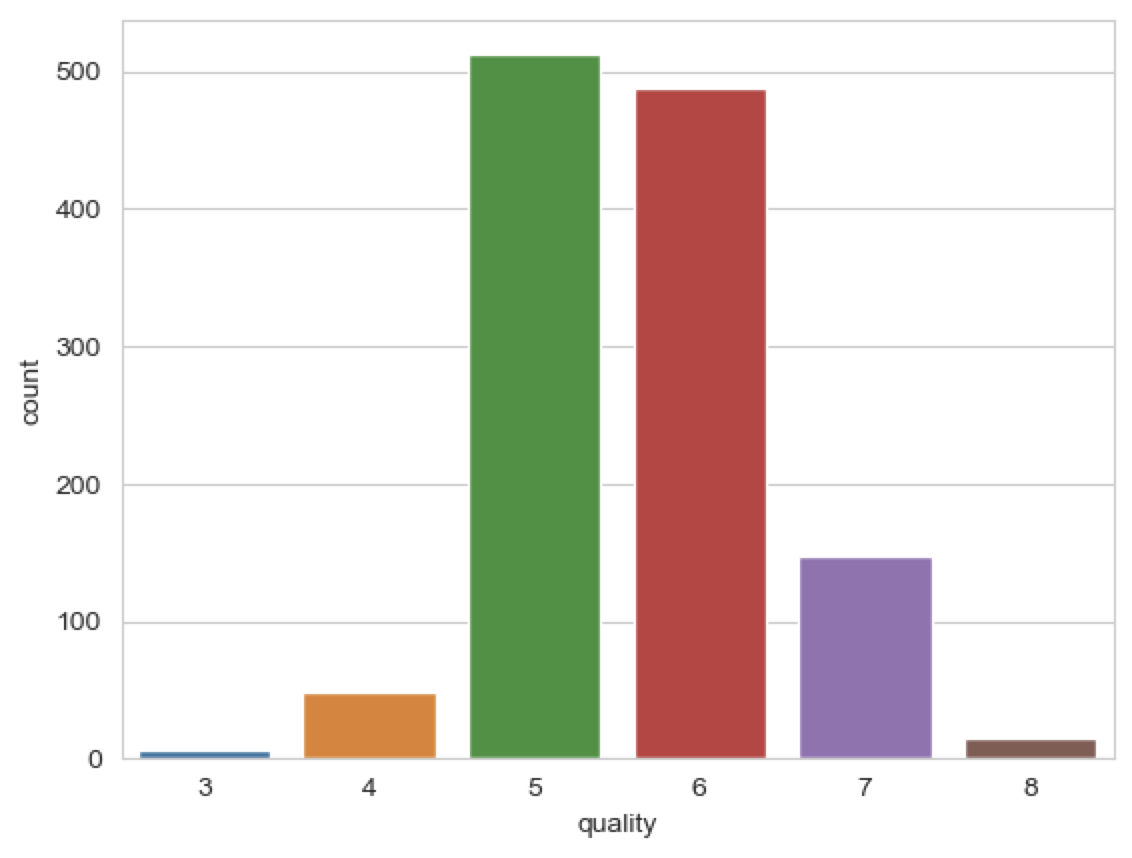
\includegraphics[scale=0.35]{quality.png}
	\caption{Quality distribution of the dataset}
	\end{center}
	\end{figure}
	
	As shown in figure 1, according to the samples, wine scores are in range from 3 to 8, and most of them have a score of 5 and 6.
	
	
	\begin{figure*}
	\begin{center}
	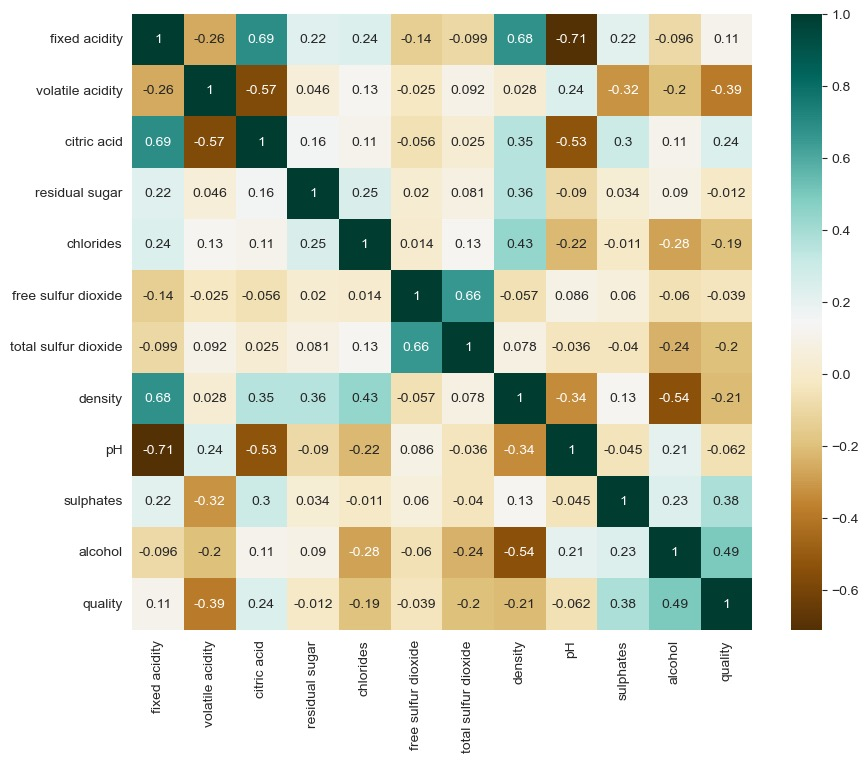
\includegraphics[width=0.9\linewidth]{heat.jpeg}
	\caption{Heat map of correlations between variables}
	\end{center}
	\end{figure*}
	
	From the heat map in figure 2, we can conclude that alcohol, volatile acidity, citric acid and sulfates have most correlated attributes with quality. Besides that, the heat map shows that alcohol has a weak positive correlation with the pH value, citric acid and density have a strong positive correlation with fixed acidity, and pH has a negative correlation with density, fixed acidity, citric acid, and sulfates.
	
	The box plots of selected feature variable over different rated quality is shown as well in figure 3 to 6, which implicates same insights on correlation between physiochemical variable and quality as summarized above.
	
	\begin{figure}[h]
	\label{fig:foo}
	\begin{center}
	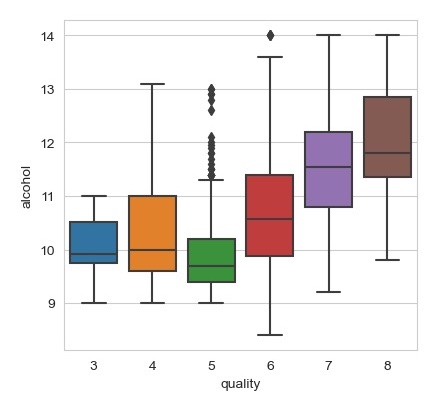
\includegraphics[scale=0.55]{a.jpg}
	\caption{Box plot of alcohol over quality}
	\end{center}
	\end{figure}
	
	\begin{figure}[h]
	\label{fig:foo}
	\begin{center}
	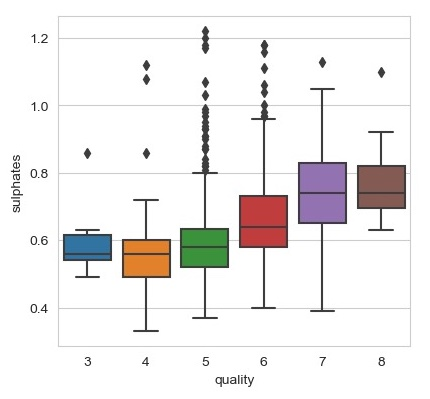
\includegraphics[scale=0.55]{s.jpg}
	\caption{Box plot of sulohates over quality}
	\end{center}
	\end{figure}
	
	\begin{figure}[h]
	\label{fig:foo}
	\begin{center}
	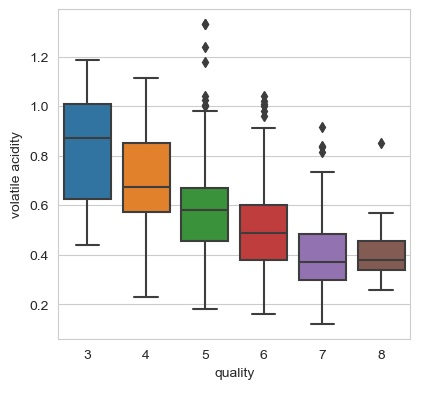
\includegraphics[scale=0.55]{v.jpg}
	\caption{Box plot of volatile acidity over quality}
	\end{center}
	\end{figure}
	
	\begin{figure}[h]
	\label{fig:foo}
	\begin{center}
	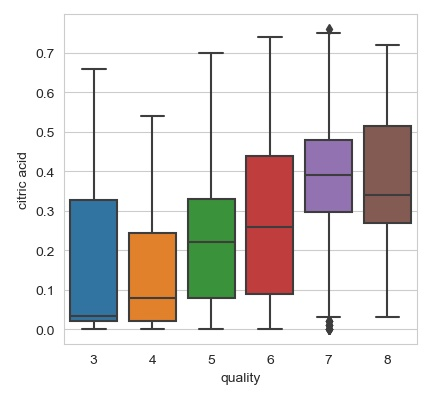
\includegraphics[scale=0.55]{c.jpg}
	\caption{Box plot of citric acid over quality}
	\end{center}
	\end{figure}
	
	




\subsection{Data Cleaning}

As the first step of the data cleaning process, duplicates are removed. Including duplicates will lead to the model overfitting this subset of points. Besides that, data leakage from validation to training data can occur  due to duplicates present in both sets, which would lead to an fictitious increase in validation performance of the model since duplicates were already learned during training.

Furthermore, outliers in the dataset are removed as the presence of outliers can affect the accuracy of statistical models. Outliers might cause the model to skew towards them, resulting in an inaccurate representation of the underlying data distribution. This can lead to overfitting, where the model fits the training data too closely and performs poorly on new, unseen data. Especially, outliers affect the performance of models based on distance measures, such as k-nearest neighbors. In KNN, outliers can be misclassified or affect the clustering of other data points, leading to inaccurate results.

\subsection{Grid Search and Weighted Features}
Grid search is a widely used hyperparameter optimization technique in machine learning that involves systematically evaluating a range of hyperparameters for a given model. This technique entails creating a grid of all possible combinations of hyperparameters and training a model for each combination. The optimal combination of hyperparameters is then determined by selecting the one that yields the highest accuracy or lowest error rate, depending on the specific problem being addressed.\\
In the present project, grid search was employed to fine-tune the hyperparameters of the Support Vector Machine (SVM) model. Specifically, the hyperparameters C and gamma were tuned using grid search to optimize the model's performance. These two hyperparameters are of particular importance in determining the efficacy of the SVM model in handling the data at hand.\cite{b5}\\
To accomplish this, a two-stage approach was used, where a broad range of C and gamma values was initially explored, followed by a more focused search of a smaller region to identify the optimal values for these hyperparameters. The implementation of the grid search algorithm used in this project is presented below:
	\begin{figure}[h]
	\label{fig:foo}
	\begin{center}
	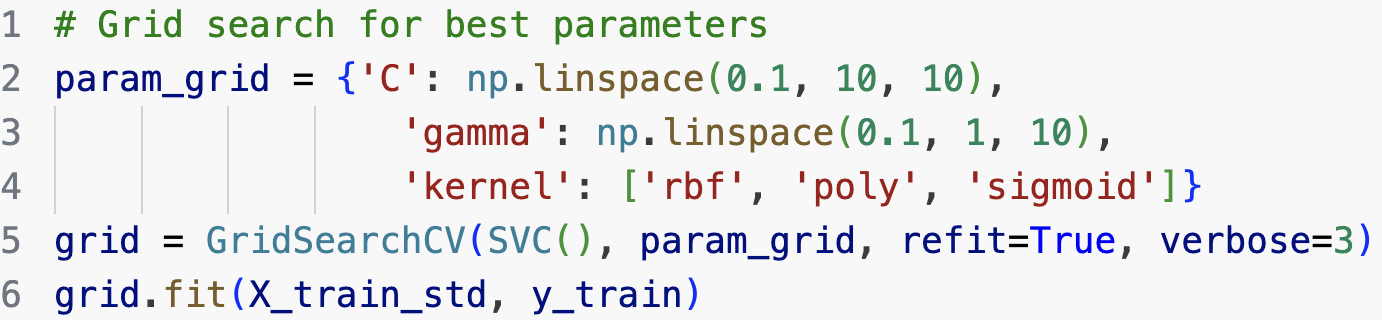
\includegraphics[scale=0.35]{gridSearch.png}
	\caption{Grid Search Code}
	\end{center}
	\end{figure}
	
\subsection{KNN}
K-Nearest Neighbors (KNN) is a supervised learning algorithm that can be utilized for both classification and regression tasks. The fundamental principle of KNN is to classify a data point based on the class labels of its K-nearest neighbors in the feature space. The choice of K, as well as the metric used for calculating distance, are important factors that influence the performance of the model.\cite{b6}\\

%KNN is a popular algorithm due to its simplicity and ease of implementation. It can easily adapt to various training datasets and requires only a few hyperparameters to be tuned, namely the value of K and the distance metric.
%
%However, there are certain limitations to KNN. Firstly, it is considered a lazy algorithm, meaning it does not perform any training during the model building process, which results in increased computational resources and memory usage. Secondly, KNN struggles with high-dimensional data inputs, since the distance metric becomes less reliable as the number of dimensions increases.

\subsection{SVM}
The Support Vector Machine (SVM) is a supervised machine learning algorithm that has gained popularity for its success in various classification tasks, including wine quality classification. SVM works by identifying a decision boundary that effectively separates the different categories of wine quality in the feature space.\\

To classify the wine quality, the SVM requires input features such as alcohol content, acidity, sugar content, and other sensory attributes. The objective of the SVM is to find a hyperplane or a linear decision boundary that can best separate the various quality categories of wine samples in the feature space. The dimensionality of this hyperplane is higher than the dimensionality of the data, and it is determined by selecting a marginal maximization hyperplane. This approach ensures that the SVM classifier is robust by calculating the distance between the hyperplane and the nearest data point for each quality category.\\

However, in cases where the data is not linearly separable, SVMs utilize kernel functions to transform the data to a higher dimensional space, which makes it linearly separable. Among the commonly used kernel functions for wine quality classification are linear, polynomial, radial basis function (RBF), and sigmoid kernels. These kernels map the data into a new feature space, where the SVM can find a hyperplane that separates the different quality categories with a good margin.\cite{b3}\\

In this project, SVM has been trained with raw data then with the standardized and cleaned data. Then Grid Search is implemented to find the best hyperparameters of C and gamma. With all the methods implemented with SVM model, the accuracy has a 10$\%$ improvement and MSE has a 33$\%$ decrement. 

\subsection{Random Forest}
Random Forest is an ensemble learning algorithm that is used for classification tasks. It works by constructing multiple decision trees and then combining their predictions to make a final prediction. The algorithm randomly selects a subset of features and a subset of training samples for each decision tree, which helps to reduce overfitting and improve the performance of the model.Also, to simplify the process, the sklearn method of $RandomForestClassifier()$ is used to classify the wine quality. (sklearn). There are eleven features imputed to the ML algorithm. Because the correlation of the wine quality is more related to some features than others, the features need to be considered differently while imputed into the machine learning algorithm. Here are the weights for each feature used in the program :{1: 10, 2: 10, 3: 69, 4: 1, 5: 1, 6: 1, 7: 1, 8: 34, 9: 10, 10: 10, 11: 80.  Those weights are estimated from the input importance of the people originally conducting the experiments.\cite{b4}\\
	\begin{figure}[h]
	\label{fig:foo}
	\begin{center}
	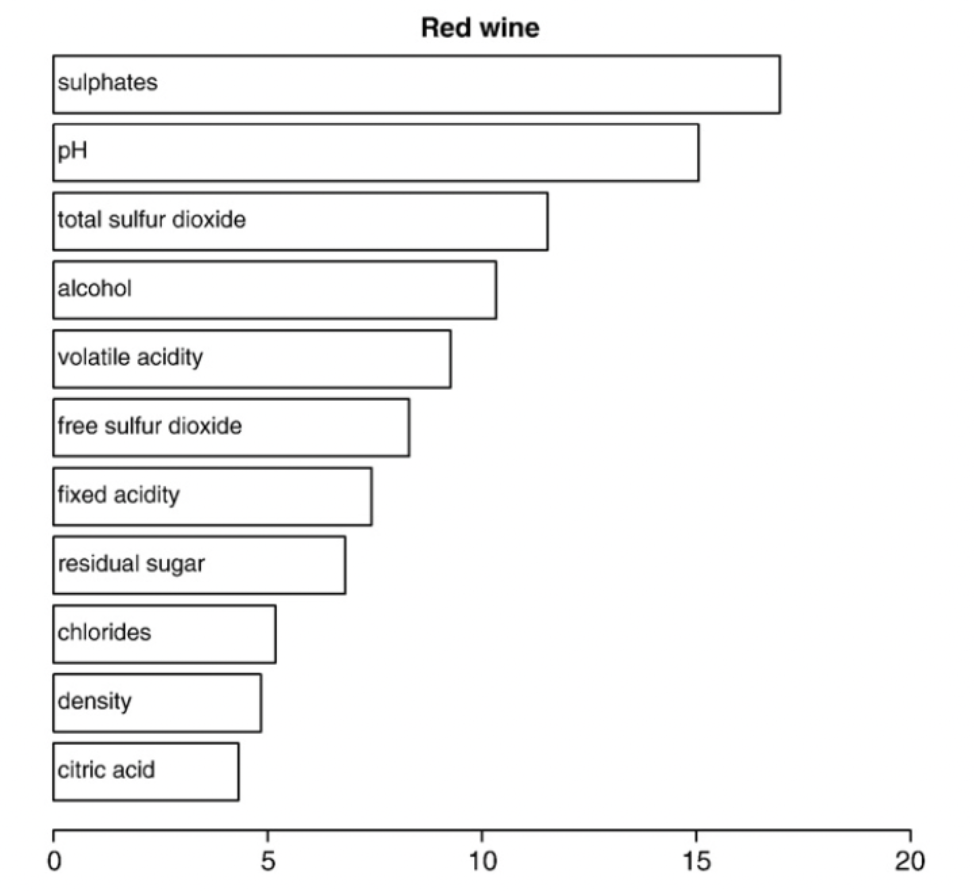
\includegraphics[scale=0.3]{redWineWeight.png}
	\caption{Red Wine Weight}
	\end{center}
	\end{figure}\\

Due to their great variety of hyperparameters, to optimize the accuracy of the method four are used which are $n estimators, max depth, random state, class weight$. The grid search is implemented to come up with the best combination of the hyperparameters, $ 'max depth': 15, 'n estimators': 700$. With given depth and number of estimators the Machine learning algorithm would output the best performances.\\
	
	
\section{Result and Analysis}
Implementing the three method mentioned above shows Random Forest does the best in all the methods. 
\subsection{KNN}
KNN method was implemented with different K number, and the accuracy result is shown below:
	\begin{figure}[h]
	\label{fig:foo}
	\begin{center}
	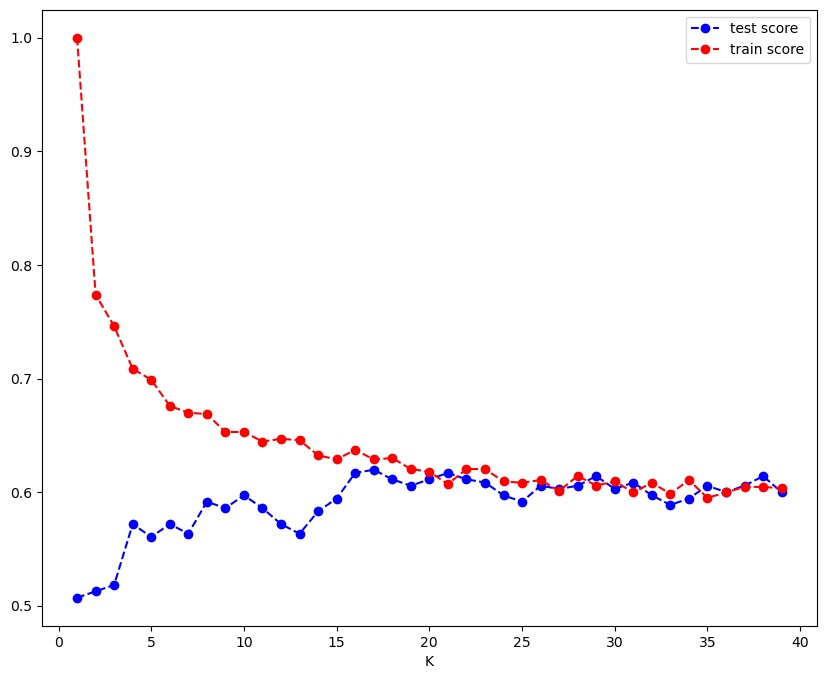
\includegraphics[scale=0.3]{KNNDiffK.jpeg}
	\caption{KNN Accuracy with Different K value}
	\end{center}
	\end{figure}
In the context of K-Nearest Neighbor (KNN) algorithm, the relationship between the value of K and the accuracy of both the training and test sets was investigated. The results showed that as K value increases, the accuracy of the training set decreases while the accuracy of the test set increases. A low value of K can cause overfitting of the data to the test set, leading to poor generalization. Conversely, increasing the K value leads to the convergence of the test accuracy and training accuracy, indicating that the KNN model is well trained. These findings suggest that the choice of K value is an important consideration when implementing the KNN algorithm, and a balance must be struck between model complexity and generalization performance. With the well-selected K value the identification situation is shown in the figure below:
	\begin{figure}[h]
	\label{fig:foo}
	\begin{center}
	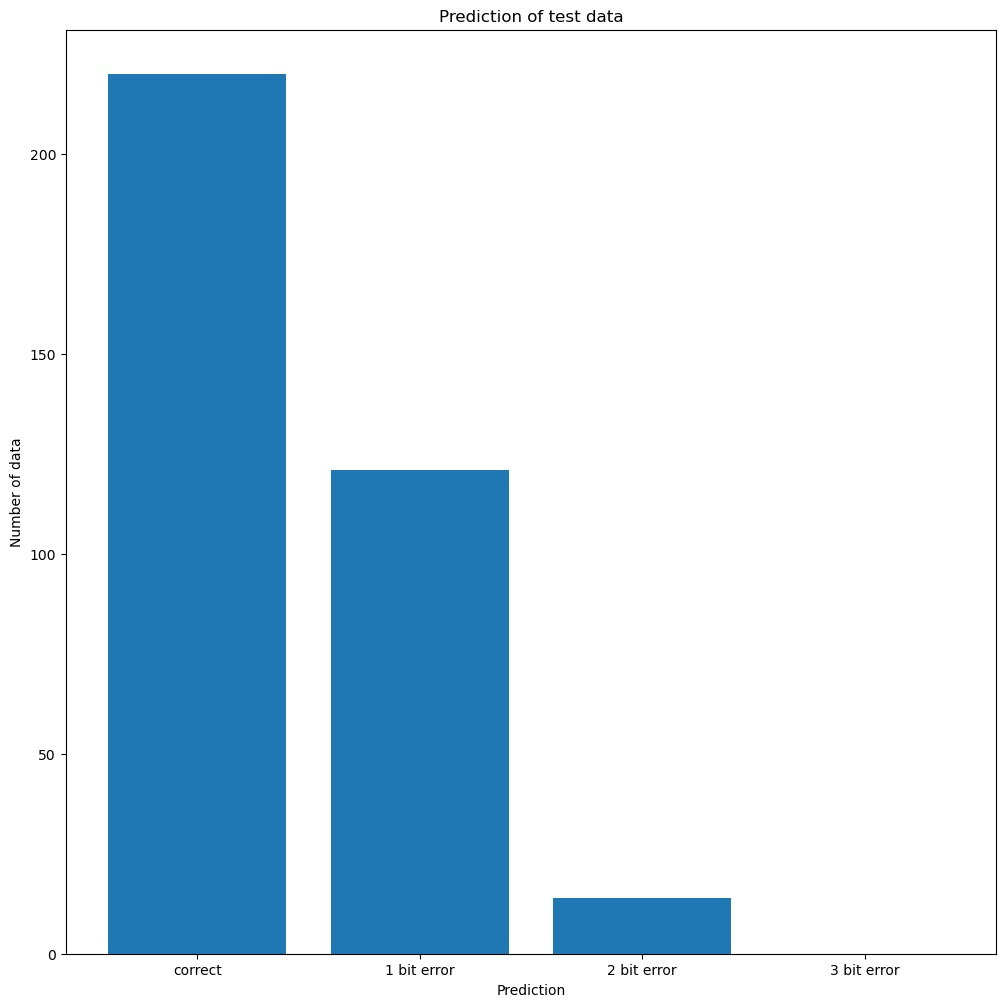
\includegraphics[scale=0.15]{KNNBar.jpeg}
	\caption{KNN Identification Situation}
	\end{center}
	\end{figure}

\subsection{SVM}
In the SVM method, no cleaning was performed on the data, and after feeding the data into the SVM model fit, an accuracy of 53$\%$ was obtained. After cleaning the data, the accuracy improved to 63$\%$. The default settings of the parameters of the SVM model were:\\

kernel='rbf', C=1.0, randomstate=0, degree=3, and gamma='auto' \\

A grid search was then performed for the hyperparameters, with C ranging from 0.1 to 10 and gamma ranging from 0.1 to 1, with three types of kernel functions, namely rbf, poly, and sigmoid. The best parameters for the grid search were found to be {'C': 2.3, 'gamma': 0.7, 'kernel': 'rbf'}. The grid search was further refined, with C ranging from 1.8 to 2.8 and gamma ranging from 0.6 to 0.8. The final optimal hyperparameters were determined to be {'C': 2.326, 'gamma': 0.705, 'kernel': 'rbf'}, and the accuracy improved from 63$\%$ to 65.87$\%$.\\
	\begin{figure}[h]
	\label{fig:foo}
	\begin{center}
	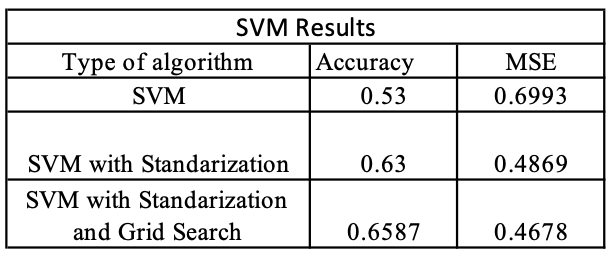
\includegraphics[scale=0.5]{SVMResult.png}
	\caption{SVM Result}
	\end{center}
	\end{figure}
	\begin{figure}[h]
	\label{fig:foo}
	\begin{center}
	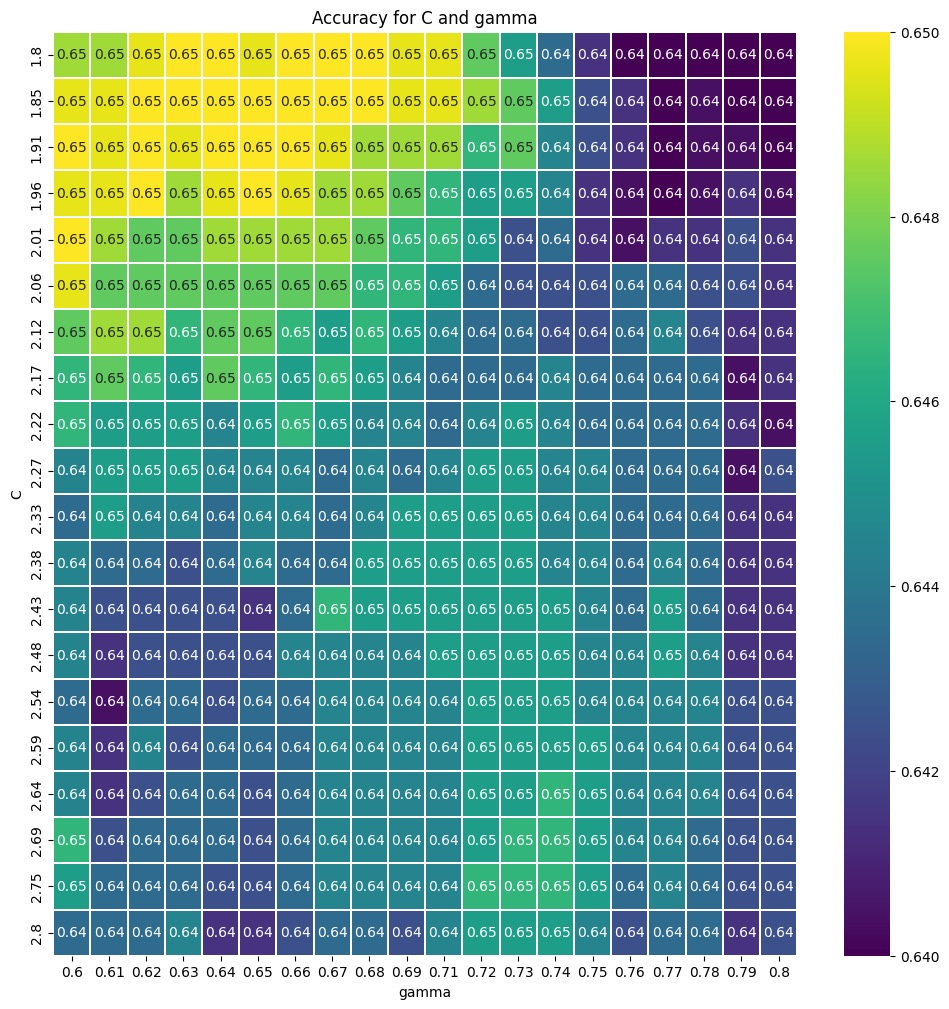
\includegraphics[scale=0.28]{SVMHeatMap.jpeg}
	\caption{SVM Grid Search Result}
	\end{center}
	\end{figure}\\
With the methods implementation, the MSE is decreasing, which is a good indicator, because MSE represents the situation of misidentification.
The mis-identification figure is shown below:
	\begin{figure}[h]
	\label{fig:foo}
	\begin{center}
	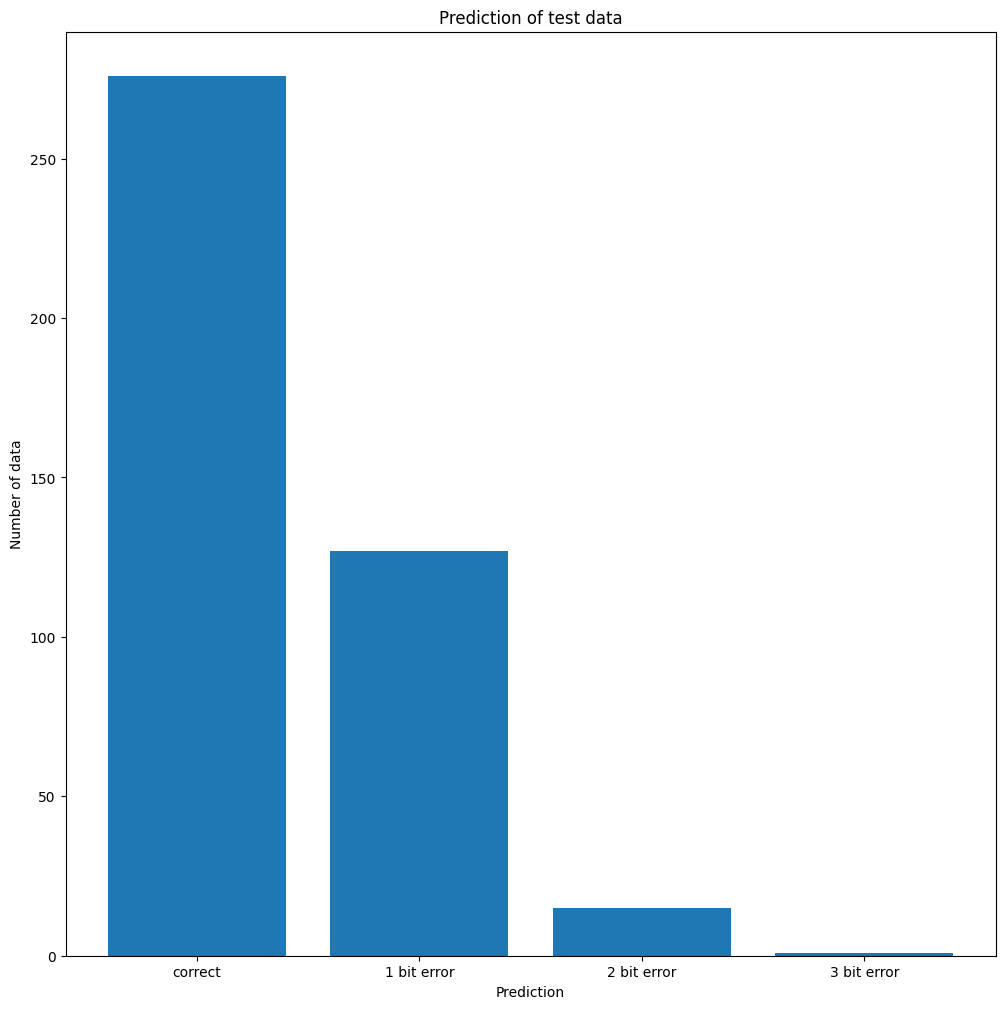
\includegraphics[scale=0.4]{SVMPrediction.png}
	\caption{SVM Prediction}
	\end{center}
	\end{figure}\\

\pagebreak

\subsection{Random Forest}
The grid search parameters demonstrated as following:
	\begin{figure}[h]
	\label{fig:foo}
	\begin{center}
	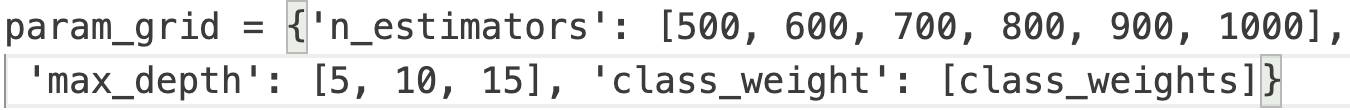
\includegraphics[scale=0.4]{RandomForestGrid.png}
	\caption{Random Forest Grid Search Code}
	\end{center}
	\end{figure}
After trials and errors, the features with the most importance are citric acid and alcohol. The density of the wine still has some weight impact to the wine but not as much. The other variables are not as important. Even the consideration chlorides, free sulfur dioxide and total sulfur dioxide would disrupt the judgment of the algorithm and lower the accuracy of the classification. \\
(1: 10, 2: 10, 3: 69, 4: 1, 5: 1, 6: 1, 7: 1, 8: 34, 9: 10, 10: 10, 11: 80)\\
All method used the random state of 3
	\begin{figure}[h]
	\label{fig:foo}
	\begin{center}
	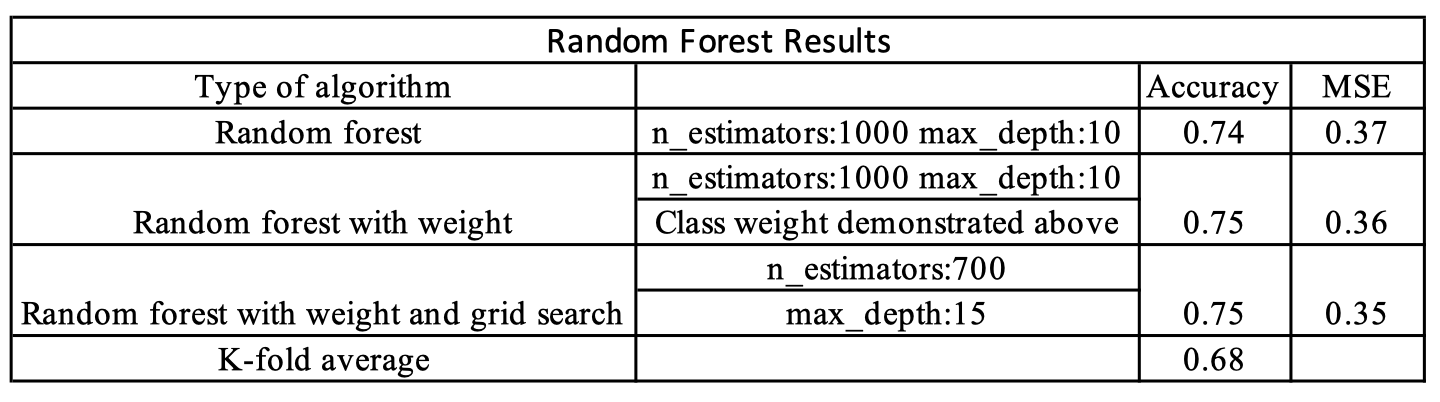
\includegraphics[scale=0.3]{randomForestResult.png}
	\caption{Random Forest Result}
	\end{center}
	\end{figure}
K-fold cross-validation is a technique used in machine learning to evaluate the performance of a model and to prevent overfitting. For cv = 10, K-fold average result is 0.68 which indicates the optimal accuracy does not deviate a lot from the average accuracy.
	\begin{figure}[h]
	\label{fig:foo}
	\begin{center}
	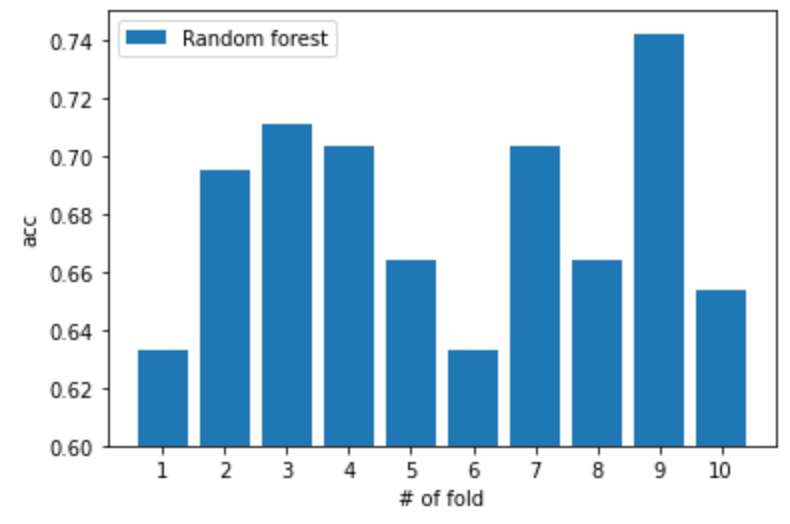
\includegraphics[scale=0.4]{RandomForestKfold.png}
	\caption{Random Forest K-fold Analysis}
	\end{center}
	\end{figure}\\
The prediction correctness is shown in figure below:\\
	\begin{figure}[h]
	\label{fig:foo}
	\begin{center}
	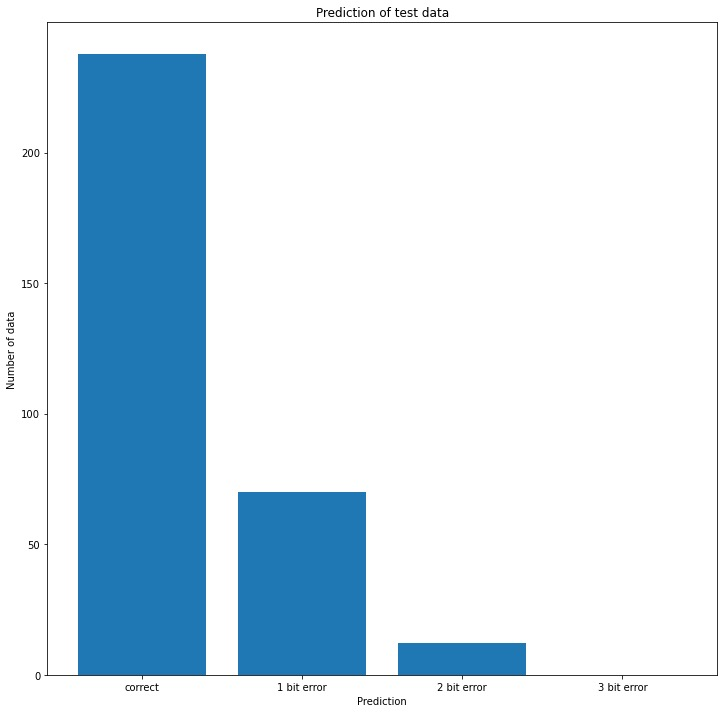
\includegraphics[scale=0.15]{RandomForestBar.jpeg}
	\caption{Random Forest Correctness}
	\end{center}
	\end{figure}\\
\pagebreak\\
	
\section{Conclusion}}

In this study, three machine learning classification methods, namely KNN, SVM, and Random Forest, were implemented to classify wines based on the UCI red-wine dataset. The KNN method had the lowest performance with an accuracy of 61.97$\%$ and a mean squared error (MSE) of 0.4985. The SVM method performed better than KNN, achieving an accuracy of 65.87$\%$ and an MSE of 0.4678. The Random Forest method outperformed the other two methods, with an accuracy of 75$\%$ and an MSE of 0.35.\\

The study also demonstrated that data cleaning and standardization were effective in improving the accuracy and lowering the MSE. These preprocessing techniques should be considered as a crucial step in machine learning classification tasks.\\

In conclusion, the Random Forest method was found to be the most effective in classifying wines based on the UCI red-wine dataset. The study highlights the importance of data cleaning and standardization in improving the accuracy and MSE of machine learning classification models. \\



\begin{thebibliography}{00}
\bibitem{b1} P. Cortez, A. Cerdeira, F. Almeida, T. Matos, and J. Reis, "Modeling wine preferences by data mining from physicochemical properties," in IEEE Transactions on Neural Networks, vol. 17, no. 5, pp. 1136-1140, Sept. 2006. doi: 10.1109/TNN.2006.176
\bibitem{b2} Wine Quality Data Set, https://archive.ics.uci.edu/ml/datasets/wine+quality
\bibitem{b3} Scikit$-$learn Support Vector Machine (SVM), https://scikit-learn.org/stable/modules/generated/sklearn.svm.SVC.html
\bibitem{b4} Scikit$-$learn Random Forest Classifier, https://scikit-learn.org/stable/modules/generated sklearn.ensemble.RandomForestClassifier.html
\bibitem{b5} Scikit-learn Grid Search Cross Validation, https://scikit-learn.org/stable/modules/generated/sklearn.model$_$selection.GridSearchCV.html
\bibitem{b6} Scikit$-$learn K$-$Nearest Neighbors Classifier, https://scikit-learn.org/stable/modules/generated/sklearn.neighbors.KNeighborsClassifier.html
\end{thebibliography}

\end{document}
